% vim: set spelllang=fr:
\chapter{Annotation en rôle sémantique basée sur la connaissance}
\label{ch:srl}


%\citep{simmons1973semantic} is the earliest work on Semantic Role Labeling.
%Already based on \citep{fillmore1968case}, it parsed a sentence into what we
% know call semantic roles. (check)

\gls{frame}

Contrairement aux autres ressources pour l'annotation en rôles sémantiques,
VerbNet couvre à la fois l'ensemble des verbes fréquents du vocabulaire tout en
étant conçu sur des préceptes robustes le rendant utile pour les tâches de
Traitement Automatique des Langues.

La tâche d'annotation en rôles sémantiques a reçu beaucoup d'attention ces
dernières années, que ce soit pour les approches supervisées ou non
supervisées. Cependant, les approches basées sur la connaissance ont été
négligées alors qu'elles apportent un compromis intéressant et sont
complémentaires par rapport aux autres approches. Ce chapitre présente un tel
système qui se veut simple et facile à reproduire. Nous montrons aussi comment
la prise en compte de la voix passive réduit le taux d'erreur de 15.7~\%, ce
qui met en avant les possibilités offertes par un tel système : une approche
simple qui facilite l'analyse des erreurs, qui n'a pas besoin d'un corpus
annoté manuellement et qui n'est pas spécifique à un domaine en particulier.

\section{Algorithme}

L'algorithme présenté est similaire à
\cite{swier2004unsupervised,swier2005exploiting}. Cependant, dix ans après, il
est important d'évaluer à nouveau cette approche pour savoir où elle se situe
par rapport à l'état de l'art et comprendre les améliorations possibles.

Le principe est d'utiliser directement les informations proposées par VerbNet.
Par exemple, VerbNet peut indiquer que dans une certaine classe, le cadre de
sous-catégorisation NP V NP correspond aux rôles Agent V Theme. Cette notation
indique que lorsque que le sujet du verbe est un syntagme nominal et que
l'objet du verbe est aussi un syntagme nominal, ils jouent respectivement les
rôles d'Agent et Theme. Dans certains cas, un même cadre de sous-catégorisation
peut correspondre à plusieurs annotations en rôles sémantiques différentes. En effet :

\begin{itemize}

    % TODO /!\ il faut déterminer la classe de toute façon
    \item si un prédicat est présent dans plusieurs classes VerbNet partageant
    les mêmes cadres de sous-catégorisation, il est possible que les annotations
    soient différentes suivant la classe considérée.

    \item certaines correspondances entre la syntaxe et la sémantique sont
    ambiguës et ne déterminent pas complètement les rôles sémantiques à utiliser.

\end{itemize}

Sans corpus annoté, ces ambiguïtés ne peuvent pas être résolues. Cependant, une
fois qu'une première série de correspondances a été effectuée, il est possible
d'utiliser les connaissances du domaine étudié pour annoter de nouveaux verbes
auparavant inaccessibles.

\subsection{Identification des arguments}

Cette première étape identifie les syntagmes amenés à recevoir un rôles
sémantique lors de l'annotation. La phrase est d'abord analysée syntaxiquement
puis certains syntagmes de la phrase sont considérés. Pour cette étape, nous
suivons \cite{lang2011unsupervised} qui propose huit règles proposant chacune
des syntagmes candidats. Ces règles génèrent trop de candidats : il faudra par
la suite soit assigner un rôle au candidat soit déclarer qu'il n'a pas de rôle
dans la phrase.

% TODO Examples
% TODO Règles
% TODO gold

\subsection{Frame matching}

Cette étape met en correspondance les syntagmes candidats précédemment
identifiés à des rôles sémantiques. Cette étape inverse deux étapes
traditionnellement utilisées dans les sytèmes d'annotation en rôles sémantiques
: \citep{gildea2002automatic,das2014frame} : l'identification des frames et
l'assignation de rôles aux arguments identifiés. En effet, nous commençons par
transformer notre liste d'arguments en construction de type VerbNet : si trois
syntagmes nominaux ont été identifiés comme arguments, dont un avant le verbe,
la représentation VerbNet de la phrase devient NP V NP NP.
% TODO confus et pas nécessairement intéressant ?
Les positions des arguments par rapport aux verbes déterminent la fonction
grammaticale de ces arguments : le premier argument est le sujet, le second un
objet direct, et le troisième un object indirect. Enfin, les syntagmes
prépositionnels sont traités à part. \citep{swier2005exploiting}.

Une fois que la phrase a été transformée en représentation Verbnet, nous
identifions toutes les classes VerbNet incluant le prédicat de la phrase afin
de comparer les frames de ces classes avec la frame identifiée dans la phrase.
Par exemple, le prédicat \textit{classify} est présent dans deux classes
VerbNet : \textit{characterize-29.2} et \textit{classify-29.10}. Les frames
possibles sont :

\begin{itemize}
    \item NP.Agent V NP.Theme (as) S\_ING.Attribute
    \item NP.Agent V NP.Theme to be ADJ.Attribute
    \item NP.Agent V NP.Theme as PP.Attribute
    \item NP.Agent V NP.Theme
    \item NP.Agent V NP.Theme as PP.Goal
    \item NP.Agent V NP.Theme in PP.Location
\end{itemize}

Prenons un example. La phrase \emph{The company also classifies short and wide
radius ruts according to their severity} est transformée en NP V NP according
PP. Dans ce cas, seuls les deux premiers arguments correspondent à des
arguments identifiés par VerbNet. Pour ces deux arguments, la correspondance
n'est pas ambiguë selon VerbNet, et le premier syntagme joue donc le rôle
d'Agent alors que le second joue le rôle de Theme. Il n'y a pas de
correspondance possible pour le troisième argument : Verbnet n'encode pas
\emph{according} comme une préposition possible alors que \emph{in} et
\emph{as} sont acceptées. Les auteurs de VerbNet travaillent actuellement sur
le problème en ajoutant des informations syntaxiques et lexicales issues de
très larges corpus \citep{bonial2013expanding}. Le résultat de ces travaux
n'est cependant pas encore disponible.

% TODO un exemple de mapping ambigu
% TODO meilleure terminologie pour ambigu/non ambigu

\subsection{Modèles de probabilité}

Maintenant qu'une partie du corpus a été annotée, nous pouvons utiliser cette
information pour annoter de nouveaux arguments ambigus. La méthode reste non
supervisée : bien que nous entraînons une forme simple d'algorithme supervisé,
nous le faisons sur des données non annotées simplement obtenues sur le corpus
existant. Dans le cas où un corpus serait inexistant, il est possible
d'abandonner cette étape ou d'alimenter les modèles de probabilité au fur et à
mesure des annotations.

Chacun de ces modèles de probabilité assigne une probabilité aux différents
rôles possibles selon les rôles identifiés de manière non ambiguë auparavant.
Une correspondance est ambigue quand deux rôles ou plus sont possibles, et est
non ambigue quand un seul rôle est possible. Différents modèles de probabilités
issus de \citep{swier2005exploiting} sont considérés.

% TODO belles formules comme dans gildea2002automatic

\paragraph{predicate-slot}

Le modèle \emph{predicate-slot} utilise l'information du prédicat et la
fonction grammaticale détectée. Par exemple, l'object direct du verbe
'négliger' sera toujours 'Theme' étant donné notre corpus
(section~\ref{srl:evaluatipn}). La précision pour ce modèle est forte, mais il
n'assigne des rôles que pour 40~\% des arguments : dans les autres cas, nous ne
disposons pas d'assez d'informations pour cette paire (prédicat, fonction
grammaticale) précise.

\paragraph{slot}

Étant donné que \emph{predicate-slot} ne donne pas de résultats dans tous les
cas, un modèle plus simple a aussi été utilisé : \emph{slot}. Ce modèle se
concentre uniquement sur la fonction grammaticale (en incluant la préposition
considérée). Par exemple, un syntagme prépositionnel \emph{of NP} correspond
dans l'ordre à Attribute, Theme et Topic dans le corpus utilisé dans cette
expérience. Dans un contexte précis, c'est le premier rôle possible qui sera
choisi. Ainsi, si l'étape précédente nous indique que Topic et Recipient sont
possibles, Topic sera choisi.

Ces deux modèles probabilistes simples sont complémentaires : un est précis
sans couvrir une large partie du corpus, alors que l'autre permet d'assigner un
rôle à chaque verbe. Cependant, la faible précision du second modèle nous
empêche de l'utiliser en l'état. % TODO que ce soit clair + future work

\section{Passive voice handling}

Error analysis revealed that passive voice was a common source of errors in our
corpus. Indeed, VerbNet does not encode the passive voice since it is a
syntactic phenomenon: it is up to the syntactic analyser to recognize that the
real subject is not where we expect it to be. Most syntactic analysers do not
handle deep structure. Handling such structures can be seen as an intermediate
step between syntactic analysis and semantic role labeling
\citep{bonfante2011modular,ribeyre2013systeme}.

We handled passive voice in the context of VerbNet by transforming VerbNet
syntactic frames temporarily whenever a passive voice is detected, that is
verbs in the past participle form which are governed by a form of the verb ``to
be''. Given a VerbNet frame such as \textit{NP.Agent V NP.Recipient NP.Theme},
we produce two transformations:

\begin{itemize}
    \item NP.Recipient V NP.Theme
    \item NP.Recipient V NP.Theme by NP.Agent
\end{itemize}

Now that the transformation is done, when faced with passive uses of verbs, we
simple use the new frames instead of the original ones to perform the mapping.
This gives better result as passive voices were always wrongly identified
(Table~\ref{table:results}).

\section{Evaluation}
\label{srl:evaluation}

L'évaluation se fait sur FrameNet, ce qui permet tout simplement d'avoir une
idée de la qualité de l'annotation en rôles sémantiques. Le mapping
VerbNet-FrameNet maintenu par le projet SemLink est utilisé.

Evaluation is currently performed against FrameNet which is one of the standard
resource for semantic role labeling. The full-text corpus is balanced,
featuring texts from multiple sources: the Wall Street Journal, the AQUAINT and
MASC corpora, and other miscellaneous texts.

\subsection{Corpora and tools}

In this experiment, we are using the full-text corpus of FrameNet 1.5, VerbNet
3.2, the VerbNet-FrameNet role mapping version
1.2.2c\footnote{\url{http://verbs.colorado.edu/semlink/1.2.2c/vn-fn/}}. Only
core arguments are considered since VerbNet often ignores the non-core FrameNet
arguments.

When working on the full semantic-parsing task, we use MST parser 0.5.0
\citep{mcdonald2006multilingual}. The parser is trained on a modified Wall
Street Journal corpus modified using NP
bracketing\footnote{\url{http://sydney.edu.au/engineering/it/~dvadas1/}} and
the LTH conversion tool for CONLL
conversion\footnote{\url{http://nlp.cs.lth.se/software/treebank_converter/}}.
Since FrameNet uses parts of the Wall Street Journal corpus, we removed six
files before training: 0558, 0089, 0456, 1778, 1286 and 1695. This ensures the
MST parser never has to parse sentences from the training set and avoids bias.
The FrameNet part-of-speech tags were converted from the BNC tagset to the WSJ
tagset using manually-defined rules (Table~\ref{table:tagset_rules}). On the
six files mentioned earlier, this reduces the number of part-of-speech tags
differences from 23\% to 3\%.

\begin{table}[hb]
    \centering
    \begin{tabular}{ccc|ccc}
        \toprule
        JJ   &$\to$& ADJ    & JJR  &$\to$& NP     \\
        JJS  &$\to$& NP     & MD   &$\to$& S      \\
        NN   &$\to$& NP     & NNP  &$\to$& NP     \\
        NNPS &$\to$& NP     & NNS  &$\to$& NP     \\
        NP   &$\to$& NP     & NPS  &$\to$& NP     \\
        PP   &$\to$& PP     & PRP  &$\to$& NP     \\  
        RB   &$\to$& ADV    & TO   &$\to$& to S   \\
        VB   &$\to$& S      & VBD  &$\to$& S      \\
        VBG  &$\to$& S\_ING & VBN  &$\to$& ADJ    \\
        VBP  &$\to$& S      & VBZ  &$\to$& S      \\
        WDT  &$\to$& NP     & \$   &$\to$& NP     \\  
        CD   &$\to$& NP     & DT   &$\to$& NP     \\
        \bottomrule
    \end{tabular}
    \caption{\protect\centering\label{table:tagset_rules}BNC to WSJ conversion rules}
\end{table}

% FUTURE SEMAFOR MXPOST/MST

\subsection{Evaluation procedure}

\begin{table*}[t!]
    \centering
    \begin{tabular}{lcccc}
        \toprule
        Task                                           & F1        & Accuracy \\
        \midrule
        FM                                             & 70.48\%   & 53.09\%  \\
        FM + predicate-slot (gold args)                & 72.02\%   & 58.28\%  \\
        FM + passive + predicate-slot (gold args)      & 76.40\%   & 62.72\%  \\
        \midrule
        Identification + FM                            & 46.75\%   & 29.12\%  \\
        Identification + FM + predicate-slot           & 46.78\%   & 33.49\%  \\
        \bottomrule
    \end{tabular}
    \caption{\protect\centering\label{table:results}Results on different tasks. FM is frame matching. Lines with \emph{passive} include the passsive voice detection. Identification is argument identification.}
\end{table*}

We feed each FrameNet sentence in the corpus to our system which performs
semantic role labeling (section \ref{sec:srl}). For each role filler annotated
in the FrameNet corpus with a verbal predicate, we use the mapping to know what
is the set of possible VerbNet roles given the FrameNet frame. This is possibly
ambiguous, mostly because a FrameNet frame can refer to multiple VerbNet
classes: we don't evaluate against those roles.

Another difficulty is that the mapping isn't complete: some VerbNet classes
cannot be mapped from FrameNet to VerbNet. Indeed, only 4605 out of 10052 roles
are mapped: we only evaluate against those frames.

We measure precision, recall, and accuracy of correct role/role filler
associations out of the FrameNet ones that have been converted to VerbNet-style
roles. 10\% of the corpus was used as a test set, while the other 90\% were
manually scanned to check for issues in our algorithm.

Table~\ref{table:results} shows results on different tasks. The first three
tasks are evaluated on gold arguments: argument identification was not needed, which
definitely helps the models. The following two tasks are evaluated on the full
frame-semantic parsing task: arguments are identified automatically based on
automatic parses. The full model is "Identification + FM + predicate-slot": it
associates argument identification, frame matching and the predicate-slot
probabilistic model.

The main takeaway is that argument identification needs to be improved
significantly to help our model reach acceptable levels of performance. The
first issue is that only around 76\% of arguments are present in our dependency
parses. The second issue is the heuristics we used for argument identification:
they need to be analysed more thoroughly or replaced with alternatives
approaches \citep{abend2009unsupervised}.

\begin{table}[ht]
    \centering
    \begin{tabular}{lccc}
        \toprule
        Model          & Precision & Coverage \\
        \midrule
        slot           & 52.45\% & 100\% \\
        predicate-slot & 68.33\% & 38.33\% \\
        \bottomrule
    \end{tabular}
    \caption{\protect\centering\label{table:probabilisticresults}Results for probabilistic models}
\end{table}

Table~\ref{table:probabilisticresults} highlights the complementary nature of
our models: the predicate slot model has better precision but lower coverage
than the slot model.

\begin{figure}[t]
    \centering
    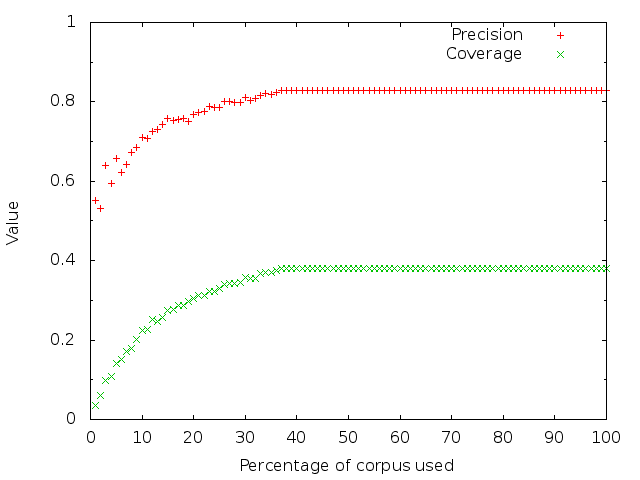
\includegraphics[width=0.45\textwidth]{fig/slot-predicate-percents.png}
    \caption{\label{fig:slot_predicate} slot-predicate model performance when training over a part of the training corpus: from 0 to 100\%.}
\end{figure}

Figure~\ref{fig:slot_predicate} highlights that we don't need the whole corpus
to attain this level of performance. This is interesting because our methods
can operate efficiently on a small domain-specific corpus and because the full
potential of this corpus is not fully realized.

\subsection{SEMAFOR comparison}

SEMAFOR \citep{das2013frame} is currently the state-of-the-art supervised
frame-semantic parser on the SemEval test sets and FrameNet full-text corpus.
It annotates all FrameNet parts-of-speech while we only concentrate on verbs.
It achieves 46.49\% F1 score on the full task, which should be compared with
the 25\% F1 score of our system.  SEMAFOR uses three stages for semantic
parsing:

\begin{itemize}
    \item target identification
    \item frame identification
    \item argument identification
\end{itemize}

As such, it cannot be compared directly with our system which does not solve
the task using the same structure. However, it is interesting to note how
important is the training data: for frame identification with gold
targets\footnote{Results for automatic targets were only given for the SemEval
2007 dataset}, the same models grows from 74.21\% to 90.51\% in F1-score for
frame identification when switching from the SemEval 2007 dataset to the
FrameNet 1.5 dataset. Likewise, for argument identification and gold
frames\footnotemark[\value{footnote}], the results grow from 48.09\% to
68.93\%. The size of the training data is extremely important, while our
approach is better suited to domain adaptation where large annotated corpora
are seldom available.

\section{Future work}

Future includes evaluating our approach on domain-specific corpora such as the
Kicktionary \citep{schmidt2009kicktionary}, the Robocup dataset
\citep{chen2008learning} or the Situated Language dataset
\citep{bordes2010towards} and compare our method with existing
domain-specific semantic role labeling work
\citep{wyner2010lexical,hadouche2011annotation,goldwasser2013leveraging}.

We also plan to incorporate more domain-specific information such as semantic
similarity between existing role fillers to detect roles that are placed in an
unusual way.

Finally, in the same way that handling the passive voice produced better
results, we plan to integrate deep structure handling to our system. A common
case of errors is coordination. When two verbs share the same subject, the
syntactic analysis should properly link from each verb to the subject. Here are
two examples: first with the verbs blunder and, then with the verbs steal and
share:

\begin{itemize}
    \item You are not fair when you belittle Sheik Bin Baz 's blunder and
          exaggerate the one by Sheik Maqdasi ...
    \item Hostile and even friendly nations routinely steal information from
          U.S. companies and share it with their own companies
\end{itemize}

More specifically, we currently plan to integrate the system from
\citep{ribeyre2013systeme} as it handles complex deep structure situations
by adding simple rules to the system to take into account new syntactic
constructions, and will allow to handle all considered deep structure links in
a cohesive way.

\section{Conclusion}

We have implemented a knowledge-based semantic role labeling system. We used
publicly available versions of data and tools which make our work easily
reproducible, now and in the future. We have started to improve the basic
algorithm with enhancements that improve its results. The current results are
probably still insufficient to improve the results of natural language
processing applications such as information retrieval or text summarization,
but the foreseeable improvements make the approach promising. The independence
of the approach with respect to annotated corpus makes it interesting even if
raw performance is as expected lower than the one of supervised approaches.
Besides the future work above, our forthcoming introduction of corpus-based
syntactico-semantic selectional restrictions is a next step.
